\chapter{Managing and transferring files}

\section{The File Manager}\label{file-manager}

After you have logged in to Globus, you will begin at the \emph{File Manager}. 
The first time you use the \emph{File Manager}, all fields will be blank.

\begin{center}
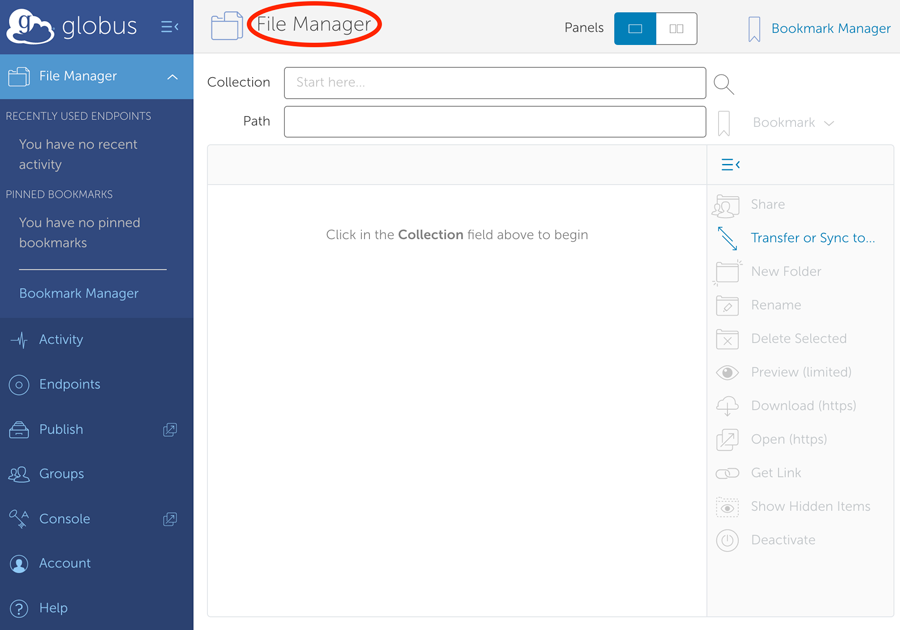
\includegraphics[width=0.5\textwidth]{img/filemanager-1.png}
\end{center}

\section{Globus Collections and Endpoints}\label{collections-endpoints}

Within Globus user data resides in a location called \gls{Globus Collection}. 
Globus Collections can be hosted on various storage and computer systems, e.g., 
HPC clusters, laptops, or cloud storage. To use a collection you only need its name. 
It is not necessary to know any details about the storage or system 
where that collection is being hosted.

An \gls{Endpoint} is a server that hosts collections. If you want to be able to 
access, share, transfer, or manage data using Globus, the first step is to create 
an endpoint on the system where the data is (or will be) stored.

To access a Globus Collection
\begin{itemize}
\item Click in the \gls{Globus Collection} field at the top of the File Manager page 
and search available collections and endpoints by typing a collection/endpoint 
name or a description. Globus will list collections with matching names.
\item Click on a collection. Globus will connect to the collection and display 
the default directory. Click the \emph{Path} field and change the path if needed. 
Globus will show the files in the new path.
\end{itemize}

\section{Transferring files}\label{file-transfer}

\begin{center}
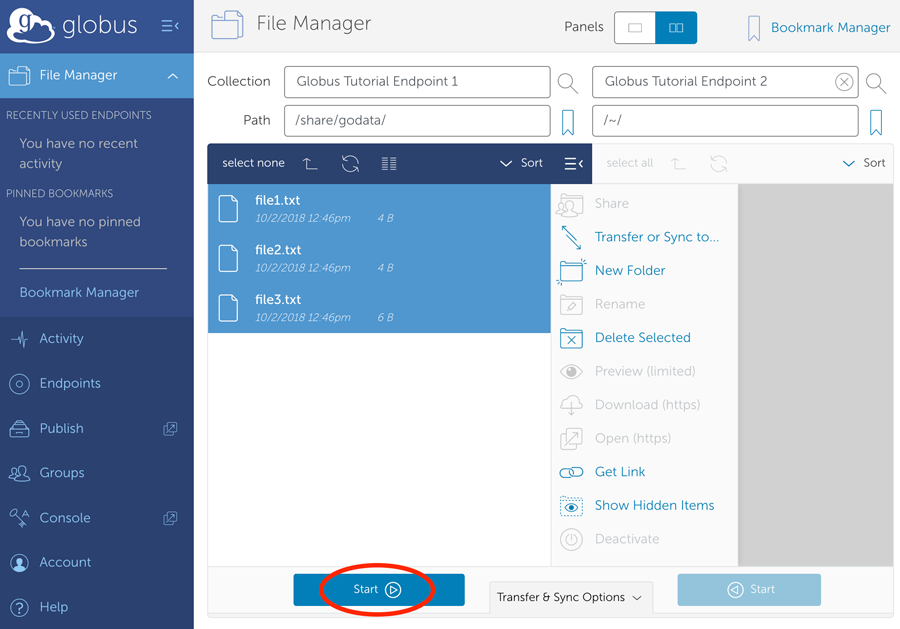
\includegraphics[width=0.5\textwidth]{img/filetransfer-2.png}
\end{center}

\begin{itemize}
\item Click \emph{Transfer} or \emph{Sync to...} in the command panel on the 
right side of the page. A new collection panel will open, with a \emph{Transfer or Sync to} 
field at the top of the panel.
\item Find and choose the second collection and connect to it as you did with the 
Globus with the first one. Click on the left first collection and select all the 
files to transfer. The \emph{Start} button at the bottom of the panel will activate.
Between the two \emph{Start} buttons at the bottom of the page, the \emph{Transfer 
and Sync Options} tab provides access to several options. By default, Globus verifies 
file integrity after transfer using checksums. Change the transfer settings if 
you would like. You may also enter a label for the transfer.
\item Click the \emph{Start} button to transfer the selected files to the 
collection in the right panel. Globus will display a green notification panel - confirming 
that the transfer request was submitted - and add a badge to the Activity item in the 
command menu on the left of the page.
You can navigate away from the \emph{File Manager}, close the browser window, and 
even logout. Globus will optimize the transfer for performance, monitor the transfer 
for completion and correctness, and recover from network errors and collection downtime.
\end{itemize}

Completed file transfers can be seen in the \emph{Activity} tab in the command menu 
on the left of the page. On the Activity page, click the arrow icon on the right to 
view details about the transfer. You will also receive an email with the transfer details.

%%% Local Variables:
%%% mode: latex
%%% TeX-master: "intro-Globus"
%%% End:
